\section{Tree Based Methods}
\subsection{Regression}
\script{303} Dabei wird das Datenset mit Bedinungen verknüpft, um anschliessend eine Vorhersage zu schätzen. Folgend ein Beispiel, wobei der Endknoten dem Mittelwert aller Werten im entsprechenden Segment ist.
\begin{center}
	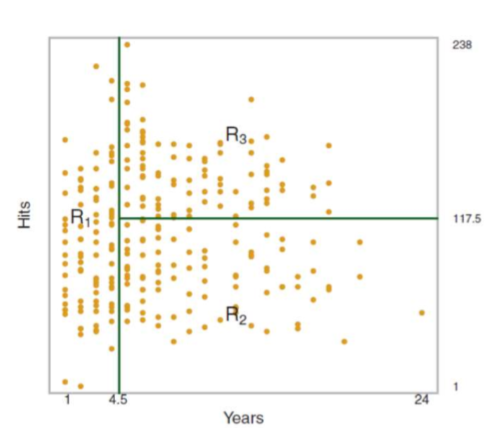
\includegraphics[width=0.3\columnwidth]{Images/tree}
	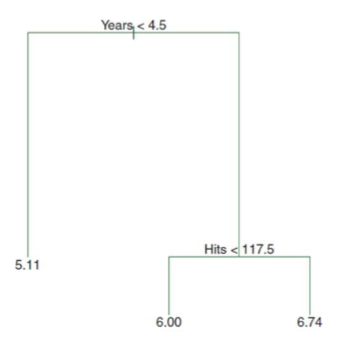
\includegraphics[width=0.3\columnwidth]{Images/tree_2}
\end{center}


\subsection{Pruning}\script{307}
Pruning schneidet die Endknoten ab, um die komplexität vom Tree zu veringern. Die Anzahl Endknoten $\left|T\right|$ sind dabei die Komplexität. Mit einem Parameter $\alpha$ können nun diese Anzahl an Subtrees definierten werden ($\alpha = 0$ = Full tree). Je grössere $\alpha$, desto grössere wird RSS. 
\begin{center}
	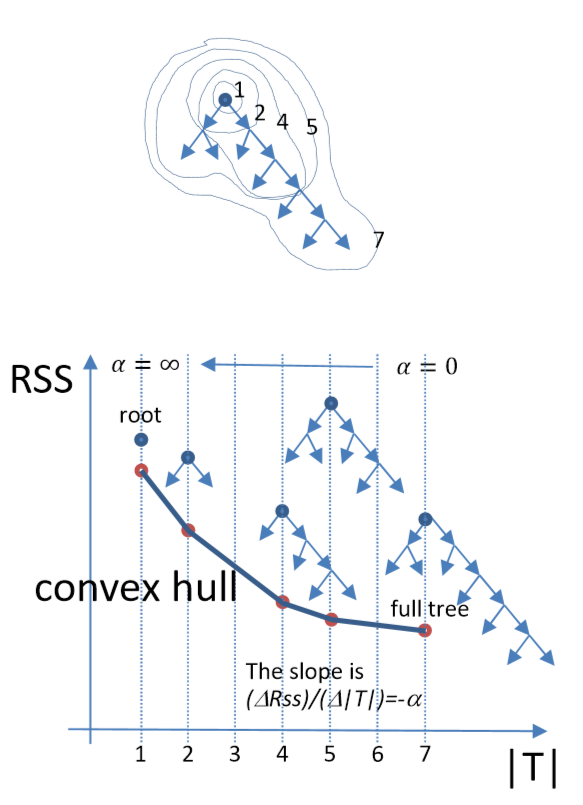
\includegraphics[width=0.5\columnwidth]{Images/pruning}
\end{center}

\subsection{Klassifizierung}\script{311}
Hier wird anstelle des RSS die maximale Fehlerrate für die optimierung verwendet.
\[
E_m = 1-\max_k(\hat{p}_{mk})
\]
$\hat{p}_{mk}$ ist die Wahrscheinlichkeit, um ein Datenpunkt von der Klasse $k$ in der $m$-th Region zu wählen. In der Praxis werden jedoch der Gini Index (auch Gini impurity) oder cross-entropie verwendet. Diese ist maximal, wenn alle Klassen gleichhäufig vorkommen.


\textbf{Gini Index $G$}
\[
G_m = \sum_{k=1}^{K}\hat{p}_{mk}(1-\hat{p}_{mk})
\]

\textbf{Cross-Entropy $D$}
\[
D_m = -\sum_{k=1}^{K}\hat{p}_{mk}\log(\hat{p}_{mk})
\]

\subsection{Random forests - Bagging}
Bagging - auch Bootstrap aggregating - ist eine Form um die Varianz zu verkleinern. Dabei wird das Trainingsset zufällig in $B$ Sets unterteilt, das Modell trainiert, um anschliessend alle Modelle mittels Durchschnitt zum finalen Modell zu verbinden.

Ein speziallfall ist Random Forests, dabei wird für jeden Split ein zufälliges Sample mit $m$ Features verwendet. Der Tree wird nur splits für diese Features haben (typisch $m=\sqrt{p}$). Wenn ein Feature sehr dominant ist, dann werden die meisten Bäume diesen als Root verwenden. Das aufteilen in andere Trees und anschliessende Mitteln wird nicht viel nützen. Beim splitten von nur $m$ Features, ist die correlation unterbrochen und wird hoffentlich bessere resultate bringen. (Hinweis: bei $m=p$, ist Random Forests gleich Bagging)